%!TEX root = ../main.tex
\documentclass{beamer} % Gliederung im Kopf, sections und subsections
\renewcommand{\baselinestretch}{1.2}\normalsize
\usetheme{default}
\setbeamertemplate{navigation symbols}{}
\setbeamertemplate{footline}[frame number]

\usepackage{tabu}
\usepackage{etex}
%\usepackage{beamerthemesplit}
%\useoutertheme[subsection=false]{smoothbars}
%\usepackage[final]{pdfpages}
\usepackage{bibentry}
\usepackage{bm}
\usepackage{bigints}
\usepackage{graphicx}
\usepackage{relsize}
\usepackage[round,longnamesfirst]{natbib}
\usepackage{bm}																									%matrix symbol
\usepackage{bbm}

\usepackage{paralist}

\usepackage{algpseudocode}
\usepackage{algorithmicx}
\usepackage{verbatim}
\usepackage{setspace}																					%Fu�noten (allgm.
\usepackage{hyperref}

\usepackage{bibentry}

\DeclareMathOperator*{\argmin}{arg\,min}
\DeclareMathOperator*{\argmax}{arg\,max}

\nobibliography*
\renewcommand{\vec}[1]{\mathbf{#1}}

\hypersetup{colorlinks=true,urlcolor=blue}														%Zeilenabst�nde)
\usepackage{threeparttable}
\usepackage{subfig}
\usepackage{epstopdf}
\usepackage{lscape}																							%Querformat
\usepackage[latin1]{inputenc}																		%Umlaute
\usepackage{graphicx}
\graphicspath{{../../material/}}

\usepackage{booktabs}
\usepackage{amsmath}
\usepackage{amssymb}
%\usepackage{uarial}

\usepackage{tabularx}
\usepackage{fancybox}																						%Boxen und Rahmen
\usepackage{appendix}
\usepackage{enumerate}

%EURO Symbol
\usepackage{tabularx}
\usepackage{longtable}																					%Mehrseitige Tabellen
\usepackage{fix-cm}
\usepackage[T1]{fontenc}
\usepackage{color,colortbl}																			%Farbige Tabellen
\usepackage{threeparttable}
\usepackage{hyperref}
\usepackage{amsfonts}

\usepackage{graphicx}
\usepackage{caption}

\usepackage{tikz}
\tikzset{
  treenode/.style = {shape=rectangle, rounded corners,
                     draw, align=center,
                     top color=white, bottom color=blue!20},
  root/.style     = {treenode, font=\Large, bottom color=red!30},
  env/.style      = {treenode, font=\ttfamily\normalsize},
  dummy/.style    = {circle,draw}
}
%\usepackage{cmbright}
\def\newblock{\hskip .11em plus .33em minus .07em}
\newcommand{\bs}{\boldsymbol}
\newcommand{\N}{\mathbb{N}}
\newcommand{\cov}{\mathrm{cov}\thin}
\newcommand{\thin}{\thinspace}
\newcommand{\thick}{\thickspace}

\newcommand{\vect}[1]{\mathbf{#1}}
\newcommand{\myfrac}[3][0pt]{\genfrac{}{}{}{}{\raisebox{#1}{$#2$}}{\raisebox{-#1}{$#3$}}}
\newcommand{\U}{\mathrm{U}}	%Uniform Distribution
\newcommand{\D}{\mathrm{D}}	%Dirichlet Distribution
\newcommand{\W}{\mathrm{W}}	%Wishart Distribution
\newcommand{\E}{\mathrm{E}}		%Expectation
\newcommand{\Prob}{\mbox{Pr}}		%Expectation
\newcommand{\Iden}{\mathbb{I}}	%Identity Matrix
\newcommand{\Ind}{\mathrm{I}}	%Indicator Function
\newcommand{\Tau}{\mathcal{T}\thin}

\newcommand{\var}{\mathrm{var}\thin}
\newcommand{\plim}{\mathrm{plim}\thin}
\newcommand\indep{\protect\mathpalette{\protect\independenT}{\perp}}
\def\independenT#1#2{\mathrel{\rlap{$#1#2$}\mkern5mu{#1#2}}}
\newcommand{\notindep}{\ensuremath{\perp\!\!\!\!\!\!\diagup\!\!\!\!\!\!\perp}}%

\newcommand{\mc}{\multicolumn}

\newcommand{\ph}{\phantom}
% weitere Optionen:
% secbar: Gliederung im Kopf, nur sections (alternativ zu subsecbar)
% handout: Produktion von Handouts, keine Animationen
\definecolor{darkblue}{rgb}{0,.35,.62}
\definecolor{lightblue}{rgb}{0.8,0.85,1}
\definecolor{lightgrey}{gray}{0.1}	%Farben mischen

%	kbordermatrix options

\makeatletter
\newcommand{\vast}{\bBigg@{4}}
\newcommand{\Vast}{\bBigg@{5}}
\makeatother
\newcommand{\indicator}[1]{\mathbbm{1}{\left\{ {#1} \right\} }}
\newcommand{\indic}{1{\hskip -2.5 pt}\hbox{1} }


\definecolor{lightgrey}{gray}{0.90}	%Farben mischen
\definecolor{grey}{gray}{0.85}
\definecolor{darkgrey}{gray}{0.65}
\definecolor{lightblue}{rgb}{0.8,0.85,1}

\renewcommand{\arraystretch}{1.5}


\usepackage{tikz}
\usetikzlibrary{trees,shapes,arrows,decorations.pathmorphing,backgrounds,positioning,fit,petri}
\renewcommand*{\familydefault}{\sfdefault}

\tikzset{forestyle/.style = {rectangle, thick, minimum width = 5cm, minimum height = 0.5cm, text width = 4.5cm, outer sep = 1mm},
	pre/.style={<-, shorten <=1pt, >=stealth, ultra thick},
	extend/.style={<-,dashed, shorten <=1pt, >=stealth, ultra thick}}
\captionsetup[subfigure]{labelformat=empty}


\newcommand{\beginbackup}{
   \newcounter{framenumbervorappendix}
   \setcounter{framenumbervorappendix}{\value{framenumber}}
}
\newcommand{\backupend}{
   \addtocounter{framenumbervorappendix}{-\value{framenumber}}
   \addtocounter{framenumber}{\value{framenumbervorappendix}}
}


% Begin Full Justification ---------------------------------------------------------

\usepackage{ragged2e}
% \usepackage{etoolbox}
\usepackage{lipsum}
\makeatletter
\renewcommand{\itemize}[1][]{%
  \beamer@ifempty{#1}{}{\def\beamer@defaultospec{#1}}%
  \ifnum \@itemdepth >2\relax\@toodeep\else
    \advance\@itemdepth\@ne
    \beamer@computepref\@itemdepth% sets \beameritemnestingprefix
    \usebeamerfont{itemize/enumerate \beameritemnestingprefix body}%
    \usebeamercolor[fg]{itemize/enumerate \beameritemnestingprefix body}%
    \usebeamertemplate{itemize/enumerate \beameritemnestingprefix body begin}%
    \list
      {\usebeamertemplate{itemize \beameritemnestingprefix item}}
      {\def\makelabel##1{%
          {%
            \hss\llap{{%
                \usebeamerfont*{itemize \beameritemnestingprefix item}%
                \usebeamercolor[fg]{itemize \beameritemnestingprefix item}##1}}%
          }%
        }%
      }
  \fi%
  \beamer@cramped%
  \justifying% NEW
  %\raggedright% ORIGINAL
  \beamer@firstlineitemizeunskip%
}

\justifying

% \apptocmd{\frame}{\justifying}{}{}

\usepackage{array}
\newcolumntype{L}[1]{>{\raggedright\let\newline\\\arraybackslash\hspace{0pt}}m{#1}}
\newcolumntype{C}[1]{>{\centering\let\newline\\\arraybackslash\hspace{0pt}}m{#1}}
\newcolumntype{R}[1]{>{\raggedleft\let\newline\\\arraybackslash\hspace{0pt}}m{#1}}



% End Full Justification ------------------------------------------------------------


%!TEX root = ../main.tex
\title{Introduction to the Econometrics of Policy Evaluation}
\author{\textbf{Philipp Eisenhauer}}
\date{\parbox{\linewidth}{\centering%
  \ldots{} background material available at \endgraf
 {\urlstyle{same}\url{{https://github.com/policyMetrics/course}}}}}



\let\otp\titlepage
%\renewcommand{\titlepage}{\otp\addtocounter{framenumber}{-1}}

\begin{document}
\maketitle


%\begin{frame}
%
%{Introduction to the Econometrics of Policy Evaluation}\label{introduction-to-the-econometrics-of-policy-evaluation}
% \ldots{} background material available at
%https://github.com/policyMetrics/course
%\subsubsection{Policy Evaluation Tasks}\label{policy-evaluation-tasks}
%
%\end{frame}

\begin{frame}
\frametitle{Policy Evaluation Tasks}
\textbf{Heckman (2008) defines three policy evaluation tasks:}

\begin{itemize}
\item
  Evaluating the impact of historical interventions on outcomes
  including their impact in terms of well-being of the treated and the
  society at large.
\item
  Forecasting the impact of historical interventions implemented in one
  environment in other environments, including their impact in terms of
  well-being.
\item
  Forecasting the impacts of interventions never historically
  experienced to various environments, including their impact on
  well-being.
\end{itemize}

\end{frame}


\begin{frame}
\frametitle{Policy Evaluation Tasks}
 The Econometrics of Policy Evaluation

\begin{itemize}
\item
 \ldots{} is important
\item
  \ldots{} is complicated
\item
  \ldots{} is multifaceted
\end{itemize}

\end{frame}

%\subsubsection{Numerous Applications}\label{numerous-applications}

\begin{frame}
\frametitle{Numerous Applications}
\begin{itemize}
\item
  Labor Economics
\item
  Development Economics
\item
  Industrial Economics
\item
  Health Economics
\end{itemize}

\end{frame}


    %\subsubsection{Numerous Effects}\label{numerous-effects}

\begin{frame}
\frametitle{Numerous Effects}

\begin{itemize}
\item
  (Local) Average Effects
\item
  Marginal Effects
\item
  Distributional Effects
\item
  Effects on Distributions
\end{itemize}

\end{frame}

   % \subsubsection{Numerous Methods}\label{numerous-methods}

\begin{frame}
\frametitle{Numerous Methods}

\begin{itemize}
\item
  Instrumental Variables
\item
  Experimental Methods
\item
  Matching
\end{itemize}

\end{frame}


%    \subsection{Unifying Framework}\label{unifying-framework}

\begin{frame}
\frametitle{Unifying Framework}

\textbf{Generalized Roy Model}
\begin{align*}
\textbf{Potential Outcomes} &\qquad \textbf{Cost} \\
Y_1 = \mu_1(X) + U_1      &\qquad C = \mu_D(Z) + U_C \\
Y_0 = \mu_0(X) + U_0      &\qquad \\
    & \\
\textbf{Observed Outcomes} &\qquad \textbf{Choice} \\
Y = D Y_1 + (1 - D)Y_0 &\qquad S = Y_1 - Y_0 - C \\
                       &\qquad D = \mathrm{I}[S > 0] \\
\end{align*}

\end{frame}


\begin{frame}
%\frametitle{Unifying Framework}
\begin{figure}[htp]\centering
\caption{Treatment Effects with Essential Heterogeneity}\label{Treatment Effects Conventional}\scalebox{0.35}{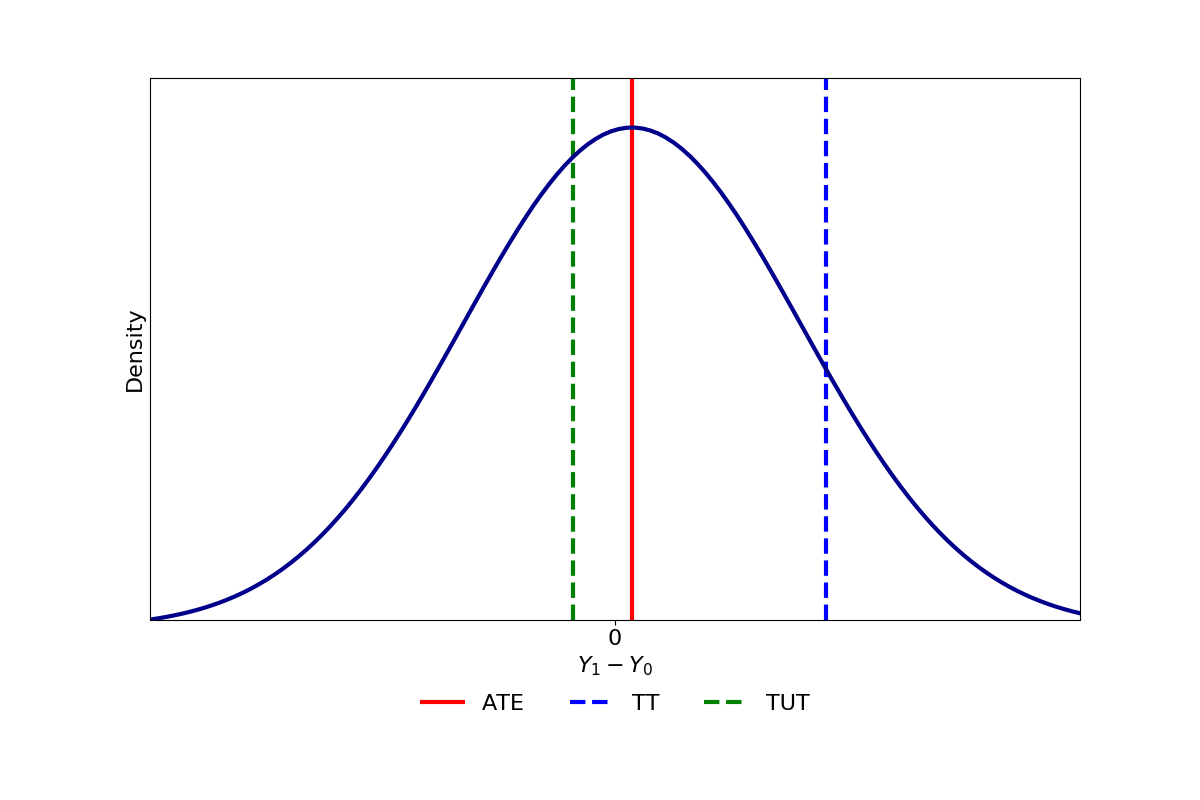
\includegraphics{fig-treatment-effects-conventional.png}}
\end{figure}

\end{frame}


\begin{frame}
\frametitle{Teaching Tool}

\begin{figure}[htp]\centering
	
\includegraphics[width=\textwidth]{fig-online-documentation.png}
%\caption{Teaching Tool}\label{Teaching Tool}
%\scalebox{0.18}{
\includegraphics{fig-online-documentation.png}}
\end{figure}

\end{frame}


    %\subsection{Lecture Plan}\label{lecture-plan}

\begin{frame}
\frametitle{Lecture Plan}
\begin{longtable}[]{@{}ll@{}}
\toprule
Date & Topic\tabularnewline
\midrule
\endhead
19/10/17 & Generalized Roy Model\tabularnewline
26/10/17 & Parameters of Interest\tabularnewline
02/11/17 & Estimation Methods\tabularnewline
09/11/17 & \emph{grmpy} Tutorial\tabularnewline
16/11/17 & Monte-Carlo Explorations\tabularnewline
23/11/17 &\tabularnewline
30/11/17 &\tabularnewline
\bottomrule
\end{longtable}

\end{frame}


 %   \subsubsection{The Mirless Review}\label{the-mirless-review}

\begin{frame}
\frametitle{The Mirless Review}

\begin{quote}
The Mirrlees Review brought together a high-profile group of
international experts and early career researchers to identify the
characteristics of a good tax system for any open developed economy in
the 21st century, assess the extent to which the UK tax system conforms
to these ideals, and recommend how it might realistically be reformed in
that direction.
\end{quote}
\end{frame}


\begin{frame}
\frametitle{Distributional Effects of Treatment}

\begin{figure}[htp]
\vspace*{-0.5cm}
\centering
\begin{minipage}[t]{0.4\textwidth}
  \centering
  \caption{The Mirless Review 1}\label{The Mirless Review 1}
  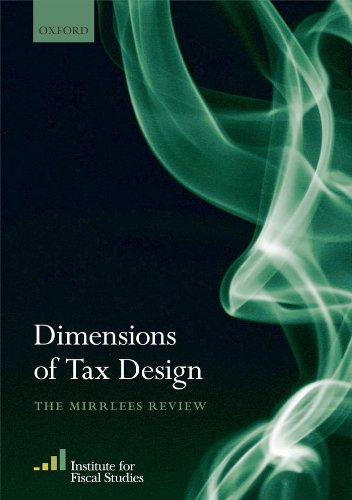
\includegraphics[width=\linewidth]{fig-mirrlees-review-1.png}
\end{minipage}%
\hfill
\begin{minipage}[t]{0.4\textwidth}
  \centering
   \caption{The Mirless Review 2}\label{The Mirless Review 2}
   
\includegraphics[width=\linewidth]{fig-mirrlees-review-2.png}
\end{minipage}
\end{figure}
\end{frame}


   % \subsubsection{Key Findings}\label{key-findings}

\begin{frame}
\frametitle{Key Findings}

\begin{itemize}
%\tightlist
\item
  \textbf{Taxation of Earnings}

  \begin{itemize}
 % \tightlist
  \item
    A single integrated benefit should be introduced to replace all or
    most of the current multiplicity of benefits, rationalising the way
    in which total support varies with income and other characteristics.
  \end{itemize}
\item
  \textbf{Indirect Taxes}
  \begin{itemize}
 % \tightlist
  \item
    VAT should be extended to nearly all spending. This would reduce
    complexity and avoid costly distortions to consumption choices.
  \end{itemize}
\end{itemize}

\end{frame}


\begin{frame}
\frametitle{Key Findings}

\begin{itemize}
%\tightlist
\item
  \textbf{Environmental Taxes}

  \begin{itemize}
 % \tightlist
  \item
    We should work towards a comprehensive system of congestion charging
    on the roads, replacing most of fuel duty.
  \end{itemize}
\item
  \textbf{Taxes on Saving}

  \begin{itemize}
 % \tightlist
  \item
    The risk-free return to saving should not be taxed, so that saving
    is not discouraged.
  \end{itemize}
\item
  \textbf{Business Taxes}
  \begin{itemize}
%  \tightlist
  \item
    The tax treatment of employment, self-employment and corporatesource
    income should be aligned.
  \end{itemize}
\end{itemize}

\end{frame}



    % Add a bibliography block to the postdoc


%!TEX root = ../main.tex
\beginbackup
%\appendix
%\begin{frame}\begin{center}
%\LARGE\textbf{Appendix}
%\end{center}\end{frame}

%------------------------------------------------------------------------------
%------------------------------------------------------------------------------
\begin{frame}\begin{center}
\LARGE\textit{References}
\end{center}\end{frame}
%------------------------------------------------------------------------------
%------------------------------------------------------------------------------
\newgeometry{margin=1cm}
\begin{frame}[allowframebreaks]\frametitle{}

\nocite{Heckman.2009e,Todd.2006,Cho.2010,Gordon.2011,Finkelstein.2012, Adam.2010,Mirrlees.2011}

\bibliographystyle{apalike}
\bibliography{../../../submodules/bibliography/literature}

\end{frame}

\backupend
\end{document}
